\documentclass{sig-alternate}
\usepackage{listings}
\begin{document}
\conferenceinfo{CSC766}{'15 Spring Raleigh, North Carolina USA}

\title{Ontology-based Knowledge Representation for PORPLE}
\subtitle{[CSC766 Final Report]}

\numberofauthors{3}
\author{
\alignauthor
Feifei Wang\\
       \affaddr{North Carolina State University}\\
       \email{fwang12@ncsu.edu}
\alignauthor
Yue Zhao\\
       \affaddr{North Carolina State University}\\
       \email{yzhao30@ncsu.edu}
\alignauthor
Xipeng Shen\\
       \affaddr{North Carolina State University}\\
       \email{xshen5@ncsu.edu}
}
\maketitle
\begin{abstract}
Data placement is important for the performance of a GPU (Graphic Processing Unit) program. However, where to place the data is a complex decision for a programmer to make. Among the recent techniques in solving data placement problem, PORPLE is a representative one. PORPLE is a portable data placement engine that uses hardware information (memory systems and processors) described by memory specification language (MSL) and software information (data access patterns) gathered from a compiler called PORPLE-C. Because of the two different representations, it is hard to share common understanding of the program, and reuse information. Providing a more general, uniform and reusable representation can make data replacement decisions more efficient, interoperable and reusable.

In this paper, we apply ontology-based techniques to systematically and formally represent both hardware information and software information used by PORPLE hoping to achieve efficiency, interoperability and reusability. Specifically, we transform the information of GPU memory systems and processors, and the data access patterns gathered by PROPLE-C to ontology which can be used by PORPLE for data replacement.
 
\end{abstract}

\terms{Compiler}

\keywords{compiler, ontology, data placement}

\section{Introduction}
Data placement is essential for the performance of a GPU (Graphic Processing Unit) program \cite{related1}. However, where to place the data depends on the hardware information of the GPU and software information of the program and its input. The hardware information of the GPU includes its memory systems and processors, while the software information means the data access patterns associated with the input to the programs. The memory systems of GPUs are becoming increasingly complex. For example, there exists more than eight types of memory (including caches) on the Tesla M2075 GPU. These memories have different size limitations, block sizes, access constraints and etc. Also, the suitable placements depend on the program inputs since different inputs to a program may lead to different data access patterns, and thus require different data placement. As a result, data placement problem is difficult but should be solved.

There have been some efforts to address the data placement problem \cite{related1, related2, related3, porple}. Among them, PORPLE \cite{porple} is a representative one since it considers various types of GPU programs. PORPLE is a portable data placement engine that takes both hardware information (memory systems and processors) and software information (data access patterns) into consideration and use them to make data placement decisions. PORPLE obtains information about memory systems and processors from memory specification language (MSL), and uses the runtime profiling to acquire the data access patterns. In such a sense, PORPLE uses two different types of representations, which makes it hard to share common understanding of the program and reuse information. Providing a more general, uniform and reusable representation can improve the efficiency, interoperability and reusability of PORPLE and potentially some other work.

There exists various techniques to represent knowledge \cite{intro2}. Recently, ontology-based knowledge bases are becoming increasingly popular. Ontology is a general-purpose modeling for knowledge resources used to define a common vocabulary and a shared understanding explicitly \cite{ontology1, ontology2}. It has been successfully used to build knowledge bases in many fields \cite{ontology3, ontology4, ontology5, ontology6, work1, work2}. Motivated by their advances, we choose ontology as the representation.

In this paper, we apply ontology-based techniques to systematically and formally represent both hardware information and software information hoping to make PORPLE more efficient, interoperable and reusable. Specifically, we transform the information of GPU memory systems and processors, and the data access patterns gathered to ontology which can be used by PORPLE for data replacement. Note that although our work is applied to PORPLE, it can also be applied to other work.

This paper is organized as follows. In Section 2, we present the motivation of our work. Section 3 illustrates the challenges of the project, our solutions, and lessons we learned. In Section 4 we explain our methodology in detail. Section 5 shows the results. Section 6 concludes this paper and discusses some possible future work.

\section{Motivation}
This work is mainly motivated by an observation that PORPLE uses two different representations for hardware information and software information. Hardware information is represented by memory specification language (MSL), which is a carefully designed small specification language. It describes the memory systems of a GPU. \ref{fig:msl} shows the MSL specification of the Tesla M2075 GPU as an example. The MSL describes the properties of a type of memory and its relations with other pieces of memory in a system. For example, the second line of the file shows the properties of globalMem. The name of the memory is globalMem, its id is 8, it is software manageable, allows read and write accesses, and etc. It also shows the relations between globalMem and L2 is that globalMem has an upper level called L2. Software information, which is data access patterns, is represented by a form defined by Chen et al. \cite{porple} \ref{fig:dap} presents one data access pattern used by PORPLE. In this file, the second line shows that the total memory access time is 64, L1 cache hit is 0, and L2 cache hit is 0.

Due to the two different representations, it is hard for them to share common understanding of the program and reuse information. In such a sense, we are motivated to choose ontology as a more general, uniform and reusable representation hoping to improve the efficiency, interoperability and reusability of PORPLE and potentially some other work.

This work is also motivated by the success of some previous work of using ontology to systematically represent, reuse, and manipulate software information, hardware information and optimization information. For example, OpenK adapts ontology-based techniques to build open and reusable knowledge bases to do program analysis and optimization in HPC. Sosnovsky et al. \cite{work1} and Ganapathi \cite{work2} et al. use ontology to teach abstract programming language. Moor et al. \cite{ontology3} and Leenheer et al. \cite{ontology4} focus on community-based evolution of knowledge-intensive systems with ontology. Tang et al. \cite{ontology5} implement a profile compiler that support ontology-based, community-grounded, multilingual, collaborative group decision making by leveraging ontology. 

\begin{figure*}
\centering
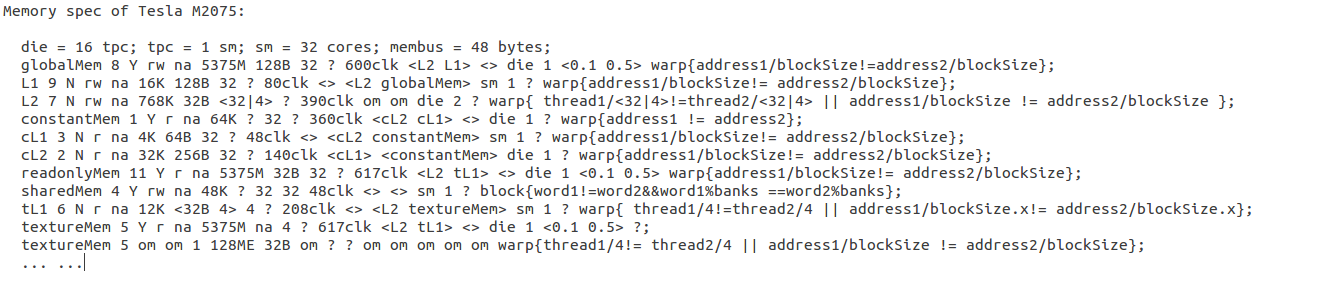
\epsfig{file=msl.png,height=4cm}
\caption{The memory specification of Tesla M2075 in MSL}
\label{fig:msl}
\end{figure*}

\begin{figure}
\centering
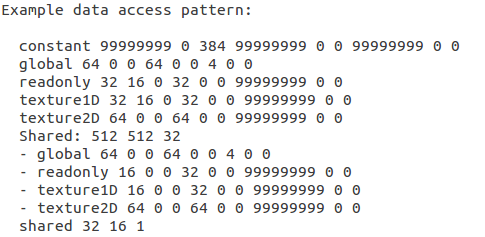
\epsfig{file=dap.png,height=4cm}
\caption{The data access pattern used by PORPLE}
\label{fig:dap}
\end{figure}

\section{Challenge, Solution and Lesson}
Transforming MSL and data access patterns used by PORPLE to ontolgoy is quite straightforward. We don't have many challenges. The main challenge is to understand ontology. In this section, we introduce the challenge to understand ontology, how we overcome them, and the lessons we learned.

\subsection{Challenge}
Ontologies have three parts: individuals, properties and classes \cite{what1}. Individuals are objects in the domain in which we are interested. Properties represent binary relations between two individuals. Objects with similar characteristics are grouped by classes. In this part we use \ref{fig:msl} as an example to illustrate the challenges. 

For the individual part, the challenge is to use unique namedIndividual for each type of memory system. For example, in the MSL for Tesla M2075, although there are four textureMems, we cannot use the same name \texttt{textureMem} for all of them. We need to make sure that every namedIndividual is unique.

For the property part, the challenge is that we need to consider inverse property. Inverse property means that if a property links individual a to individual b then its inverse property will link individual b to individual a \cite{what1}. For example, if globalMem has an upper level that is L2, then L2 should have a lower layer that is globalMem. 

For the class part, the challenge is to consider some characteristics that is not so obvious. For example, L1 is a sub-class of Cache is obvious. However, we need to consider that M2075 is a sub-class of Tesla, and M2075Processor is a sub-class of Processor.

\subsection{Solution}
Our solution is to use Protege \cite{protege} to generate ontology files, and then learn from those generated files. By learning from Protege, we learn to define classes and arrange them in a hierarchy (sub-class hierarchy). We consider Tesla, M2075, Processor, scope, GlobalMemory, ConstantMemory, TextureMemory, Cache and etc. We also learn to define the properties that should be assigned to each class and give them values. We also learn to define individuals.

\subsection{Lesson}
The lesson is that when creating ontology, we must think comprehensively.

\section{Implementation}
We have designed two implementations for MSL and data access patterns. We first introduce the implementation for MSL in detail, and then describe the implementation for data access patterns.

\subsection{MSL}
When transforming MSL to ontology, we create individuals and then enumerate properties about them, and assert class descriptions about them.

We first need to add various type of memory systems� to our ontology. For example, globalMem, constantMem, sharedMem, are regarded as individuals. We use namedIndividuals since they are given an explicit name that can be used in any ontology to refer to the same object. 

We then enumerate the properties of individuals. By parsing the input file, we can get the information we need to create properties. We use two kinds of properties. (item?) One is called the ObjectPropertyAssertion that allows one to state that an individual is connected by an object property expression to an individualIn. The other one is called the DataPropertyAssertion axiom allows one to state that an individual is connected by a data property expression to a literal. In MSL, we can get information about ObjectPropertyAssertion such as ... Also, we can get information about DataPropertyAssertion such as ...

In the end, we define sub-class hierarchy to state that an individual is an instance of a particular class.

\subsection{Data Access Patterns}
Transforming data access patterns to ontology is quite easy since the semantics of data access patterns is simple. We only need to create ....and for each number not begins with 9 (designed by Chen et al. \cite{porple}) ... We should note that we use - to get off-chip memory access times.

\section{Results}

The individual a:Peter can be used to represent a particular person. It can be used in axioms such as the following one:

ClassAssertion( a:Person a:Peter )	Peter is a person.

DataPropertyAssertion( a:hasAge a:Meg "17"^^xsd:double )	Meg is seventeen years old.
The first axiom states that all values of the a:hasAge property must be in the value space of xsd:integer, but the second axiom provides a value for a:hasAge that is equal to the floating-point number 17. Since floating-point numbers are not contained in the value space of xsd:integer, the mentioned ontology is inconsistent.

bjectPropertyAssertion( a:hasBrother a:Chris a:Stewie )	Stewie is a brother of Chris.

http://protege.stanford.edu/publications/ontology_development/ontology101.html

\section{Conclusion and Future Work}

Classes can be organized into superclass-subclass hierarchy and they are described or defined by the relationships that individuals participate in.


\section{Acknowledgments}
This section is optional; it is a location for you
to acknowledge grants, funding, editing assistance an

\bibliographystyle{abbrv}
\bibliography{sigproc} 

\end{document}
\begin{thebibliography}{1}

\end{thebibliography}
